\documentclass[main.tex]{subfiles} 
\begin{document}

\begin{figure}[h!]
\centering
    \begin{subfigure}{.5\textwidth}
    \centering
    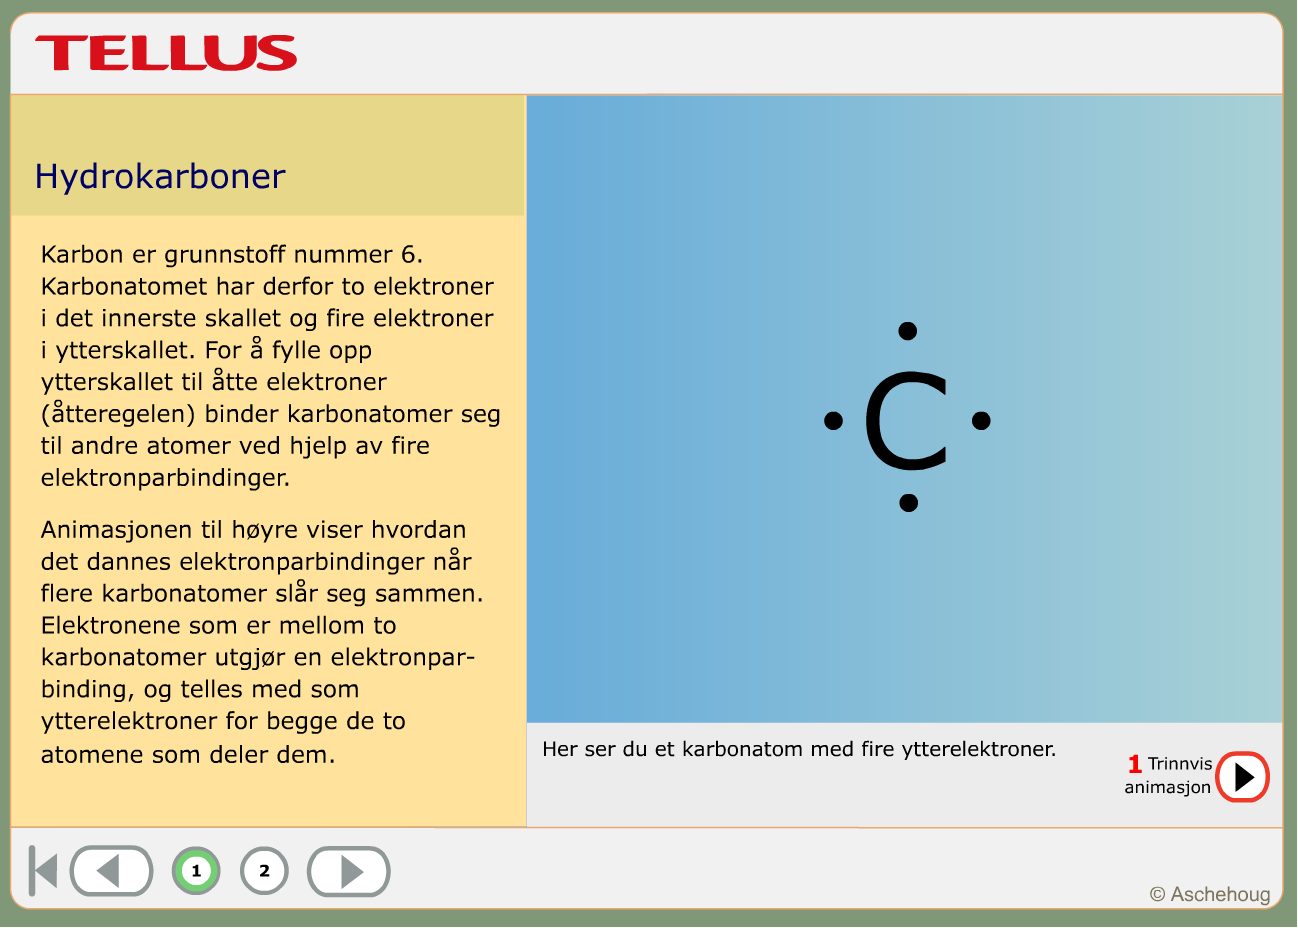
\includegraphics[scale = 0.20]{../figures/lokus1.png}
    \end{subfigure}%%
    \begin{subfigure}{.5\textwidth}
    \centering
    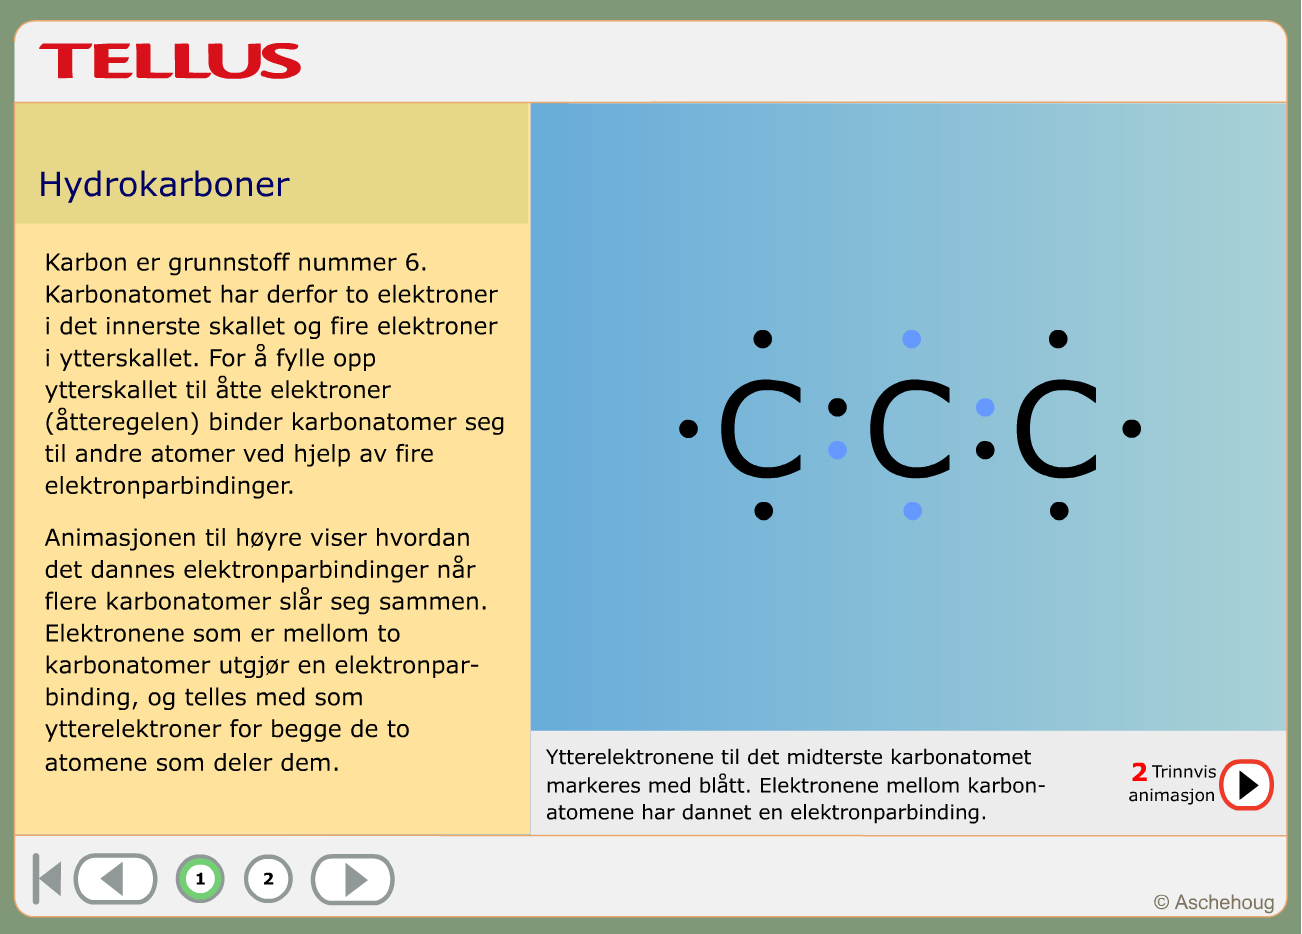
\includegraphics[scale = 0.199]{../figures/lokus2.png}
    \end{subfigure}
    \begin{subfigure}{.5\textwidth}
    \centering
    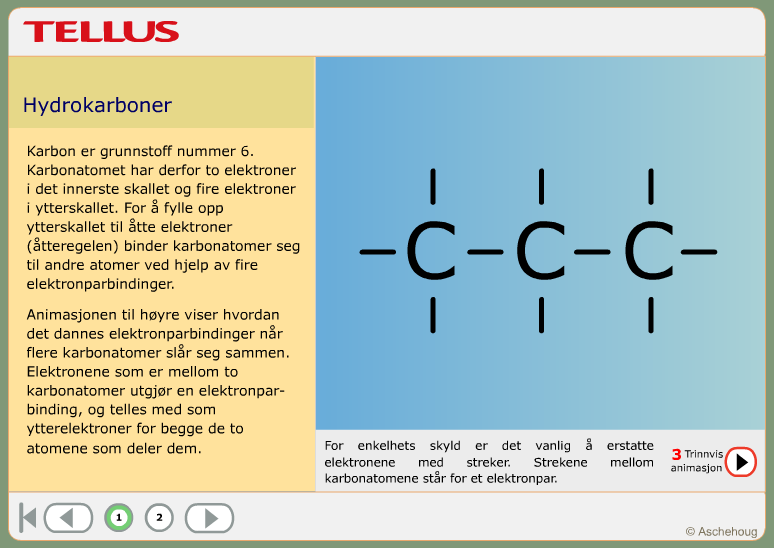
\includegraphics[scale = 0.34]{../figures/lokus3.png}
    \end{subfigure}%%
    \begin{subfigure}{.5\textwidth}
    \centering
    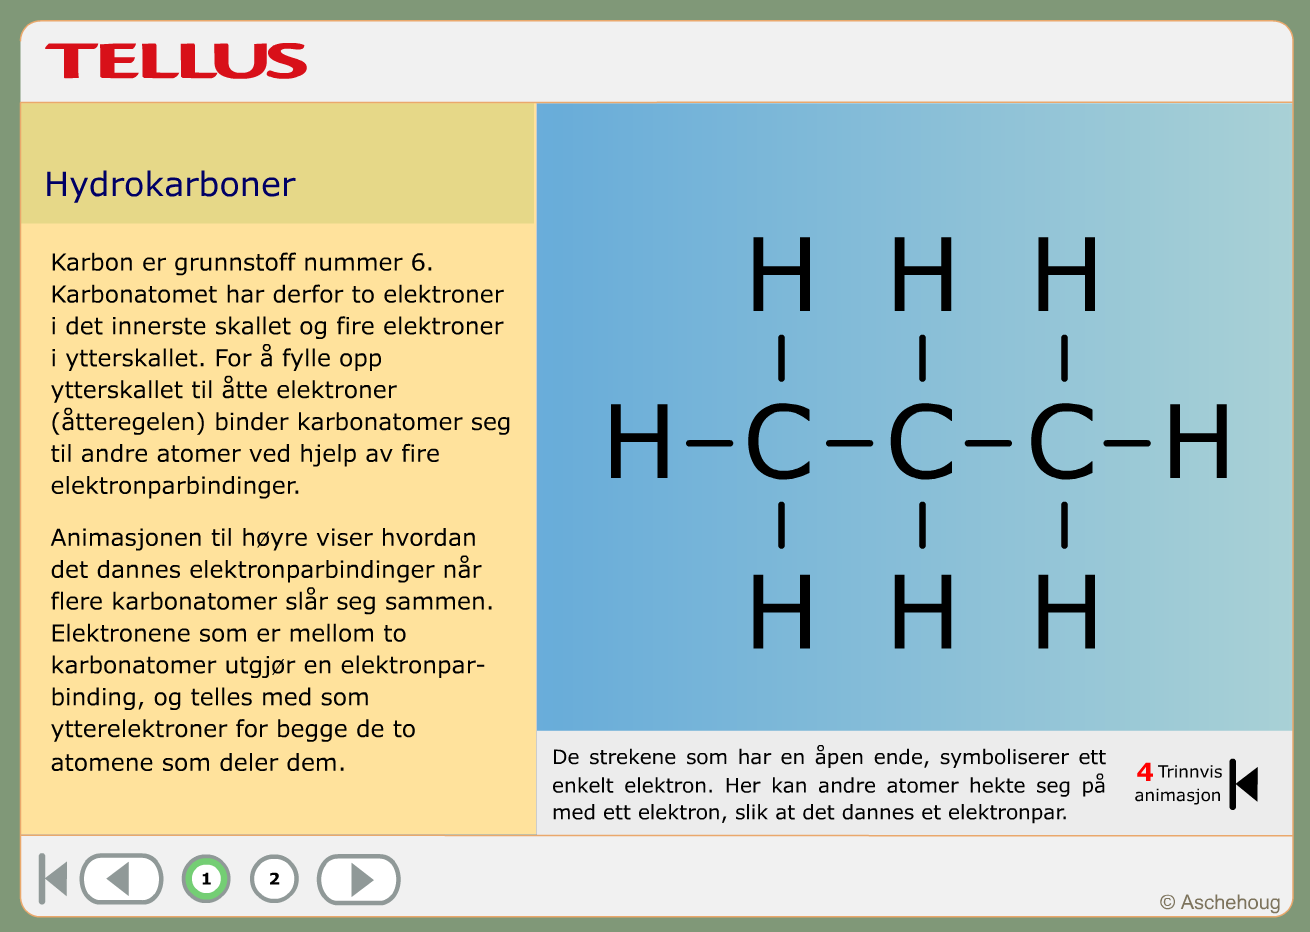
\includegraphics[scale = 0.199]{../figures/lokus4.png}
    \end{subfigure}
    \caption{Interaktiv forklaring for elektronparbindinger når flere karbonatomer slår seg sammen. Kilde: 
    \protect\url{http://www3.lokus.no/flashEmbedder.jsp?contentItemId=52275952&selectedLanguageId=1&title=hydrokarboner}}
    \label{fig:lokus}
\end{figure}

\begin{figure}[h!]
\centering
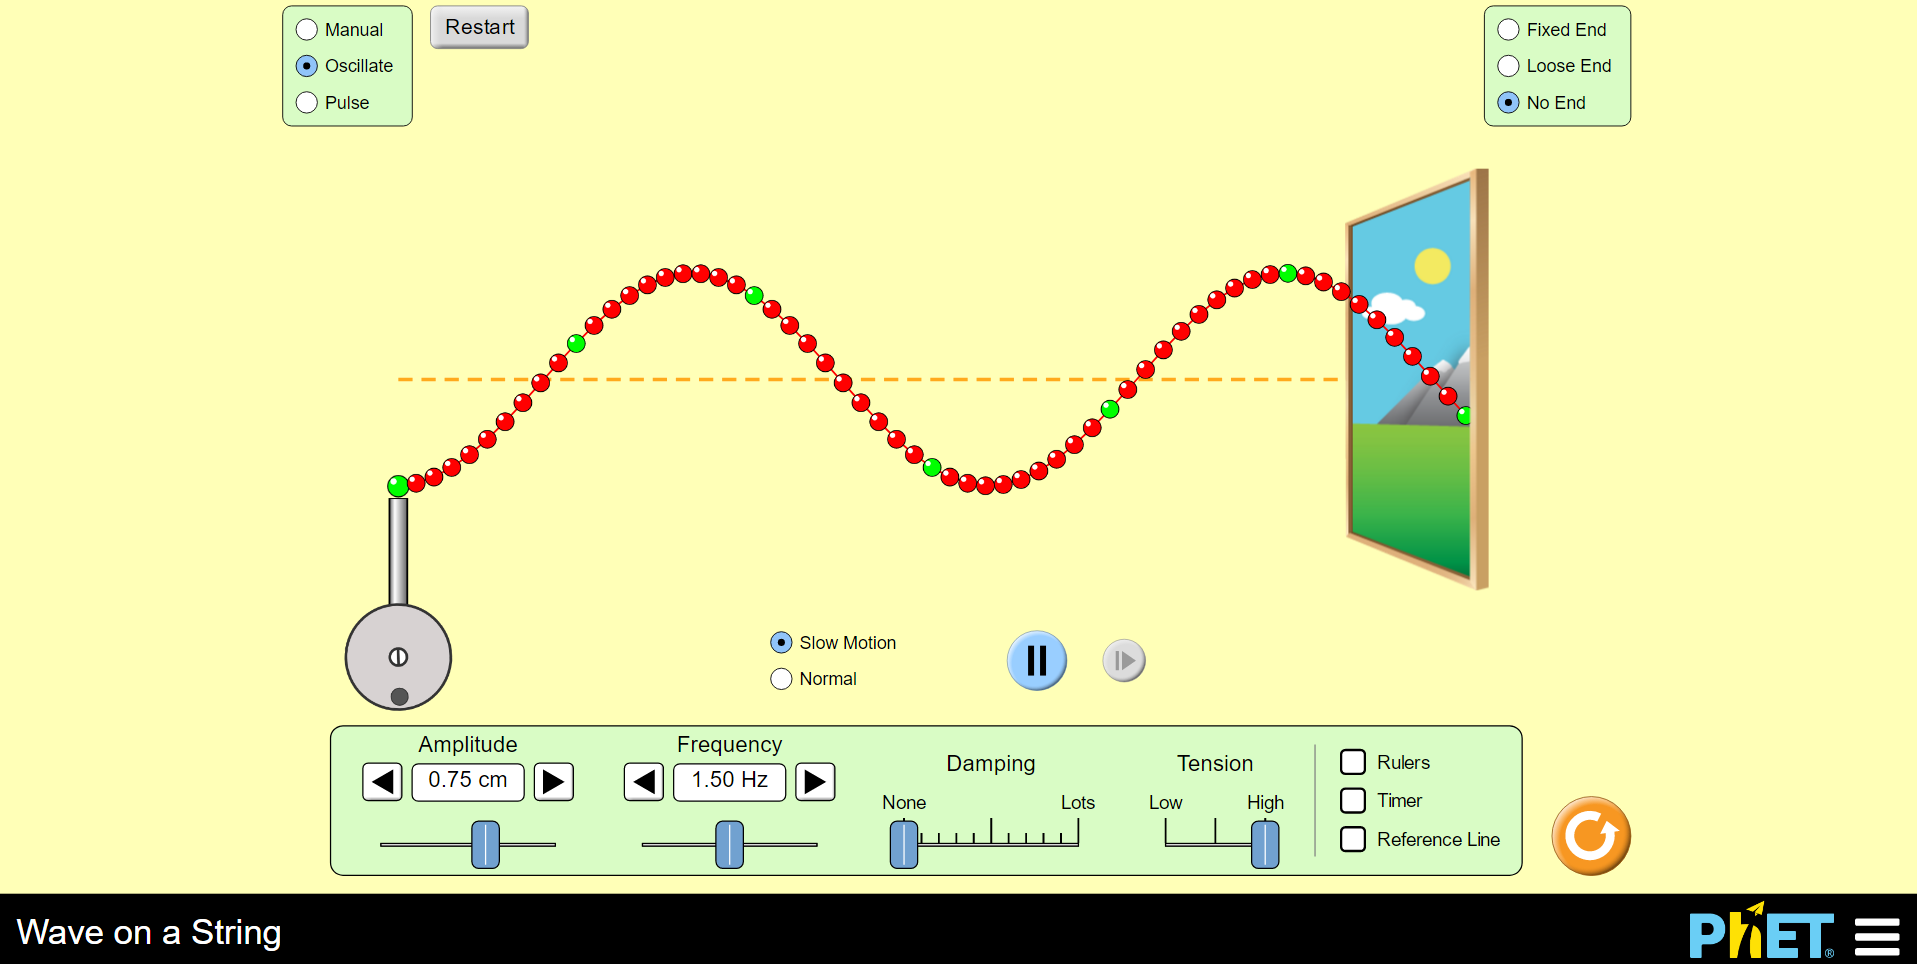
\includegraphics[scale = 0.25]{../figures/wave.png}
\caption{Interaktiv simulering av en oscillerende streng. Kilde: 
\protect\url{https://phet.colorado.edu/sims/html/wave-on-a-string/latest/wave-on-a-string_en.html}}
\label{fig:wave}
\end{figure}


\end{document}